\renewcommand\thesection{XII}
\section{Induction Électromagnétique, et Inducteurs}

\begin{multicols*}{2}
    \subsection{Conditions pour créer des courants induits}
    
    \begin{itemize}
        \item Lorsqu'un champ magnétique au travers d'une boucle de conducteur varie.
        \item Pour une boucle de conducteur flexible située dans un champ magnétique constant et uniforme: lorsque l'aire délimitée par cette boucle est modifiée.
        \item Pour une boucle de conducteur d'aire constante: lorsque l'on fait tourner la boucle par rapport à la direction du champ.
    \end{itemize}
    
    \subsection{Lois de Faraday et Lenz}
    
    \subsubsection{Loi de Faraday}
    
    \[ | \xi _{\text{ind}} | = \left| \frac{d \varPhi _B}{dt}\right| \]
    Avec $\varPhi_B$ étant le flux magnétique en Weber ($Wb$).
    \[1 Wb = 1 T \cdot 1 m^2 \]
    
    \paragraph{Boucle Uniforme et Plane}
    
    \[ \varPhi_B = A \cdot B \cdot \cos\vartheta \]
    \begin{center}
        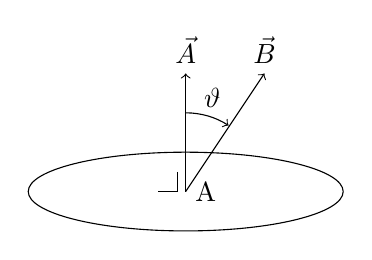
\begin{tikzpicture}[scale=0.5, smooth]
            \draw (0,0) ellipse (4 and 1) node[right] {A};
            \draw[->] (0, 0) -- (0, 3) node[above] {$\vec A$};
            \draw[->] (0, 0) -- (2, 3) node[above] {$\vec B$};
            \draw[->] (0, 2) arc (90:57:2) node[pos=0.6, above] {$\vartheta$};
            \draw (-0.2, 0.5) -- (-0.2, 0) -- (-0.7, 0.0);
        \end{tikzpicture}
    \end{center}
    
    En définissant $\vec A$ comme le vecteur perpendiculaire à la boucle de longueur A:
    
    \[ \Rightarrow \varPhi_B = \vec A \cdot \vec B \qquad \text{pour $\vec B$ uniforme} \]
    
    \paragraph{Champ non Uniforme/ Boucle non Plane}
    
    \[ \varPhi_B = \int \vec B \cdot d \vec A \]
    
    \subsubsection{Loi de Lenz}
    
    Le sens du courant induit est tel que le champ magnétique qu'il produit s'oppose à la variation de flux qu'il produit.
    \begin{multicols}{2}
        \begin{center}
            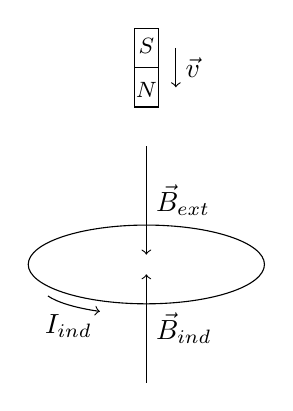
\begin{tikzpicture}[scale=0.5]
                \draw (0,0) ellipse (3 and 1);
                \draw[->] (0, -3) -- (0, -0.25) node[right, pos=0.5] {$\vec B_{\text{ind}}$};
                \draw[->] (0, 3) -- (0, 0.25) node[right, pos=0.5] {$\vec B_{\text{ext}}$};
                \draw[->] (-2.5, -0.8) arc (200:240:3 and 0.75) node[below, pos=0.5] {$I_{\text{ind}}$};
                \draw (-0.3, 5) -- (-0.3, 6) -- (0.3, 6) node[below, pos=0.5] {\footnotesize $S$} -- (0.3, 5) -- (-0.3, 5) -- (-0.3, 4) -- (0.3, 4) node[above, pos=0.5] {\footnotesize $N$} -- (0.3, 5);
                \draw[->] (0.75, 5.5) -- (0.75, 4.5) node[right, pos=0.5] {$\vec v$};
            \end{tikzpicture}
        \end{center}
        
        \begin{center}
            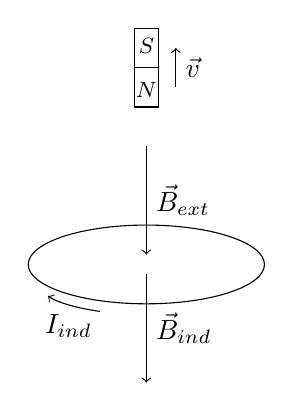
\begin{tikzpicture}[scale=0.5]
                \draw (0,0) ellipse (3 and 1);
                \draw[<-] (0, -3) -- (0, -0.25) node[right, pos=0.5] {$\vec B_{\text{ind}}$};
                \draw[->] (0, 3) -- (0, 0.25) node[right, pos=0.5] {$\vec B_{\text{ext}}$};
                \draw[<-] (-2.5, -0.8) arc (200:240:3 and 0.75) node[below, pos=0.5] {$I_{\text{ind}}$};
                \draw (-0.3, 5) -- (-0.3, 6) -- (0.3, 6) node[below, pos=0.5] {\footnotesize $S$} -- (0.3, 5) -- (-0.3, 5) -- (-0.3, 4) -- (0.3, 4) node[above, pos=0.5] {\footnotesize $N$} -- (0.3, 5);
                \draw[<-] (0.75, 5.5) -- (0.75, 4.5) node[right, pos=0.5] {$\vec v$};
            \end{tikzpicture}
        \end{center}
    \end{multicols}
    
    \subsubsection{Faraday et Lenz combinées}
    
    \[ \xi_{\text{ind}} = -\frac{d \varPhi _B}{dt} \]
    
    \paragraph{Cas d'un bobinage de N spires}
    
    \begin{center}
        \begin{circuitikz}[scale=0.5]
            \draw (0,0) to [L] (6,0);
            \draw (2.2, -0.5) -- (2.2, -0.75) -- node[below, pos=0.5] {$N$} (3.8, -0.75) -- (3.8, -0.5);
        \end{circuitikz}
    \end{center}
    Si $\varPhi_B$ dans chaque spire est identique, alors chaque spire est siège d'une f.é.m.
    \[ \xi_{\text{ind}} = -N \frac{d\varPhi_B}{dt} \]
    
    \subsection{Inductance et Inducteurs}
    
    \subsubsection{Inductance Mutuelle}
    \begin{center}
        \begin{circuitikz}
            \ctikzset{resistors/scale=0.75}
            \ctikzset{inductors/scale=1.5, inductors/coils=8}
            \draw (-1, 0) to [vsourcesin] (-3, 0) to [R] (-3, 2) to (-3, 3) to [L = $1$] (-1, 3) to (-1, 0);
            \draw (0, 1) to (0, 3) to [L = $2$] (2, 3) to (2, 1);
            \draw[dashed] (0, 0.27) -- (0, 1);
            \draw[dashed] (2, 0.27) -- (2, 1);
            
            \draw[<->] (-3, 2) -- (-1, 2) node[below, pos=0.5] {$\xi_1$};
            \draw[<->] (0, 2) -- (2, 2) node[below, pos=0.5] {$\xi_2$ {\footnotesize(induit)}};
            
            \draw[->] (-0.5, 3.15) -- (2.5, 3.15) node[above] {$\vec B_1$};
        \end{circuitikz}
    \end{center}
    
    Avec $\varPhi_{21}$ le flux magnétique créé dans chaque spire de la bobine 2 par le champ magnétique variable $\vec B_1$ créé par le courant $I_1$ circulant dans la bobine 1. D'où $N_2\varPhi_{21}$ est le flux magnétique traversant la bobine 2 entière.
    
    \[ \xi_2 = - \frac{d(N_2\varPhi_{21})}{dt} = -N_2 \frac{d\varPhi_{21}}{dt} \]
    \[ \text{En posant} \qquad N_2 \varPhi_{21} = MI_1 \]
    
    Avec $M$ la constante de proportionnalité d'inductance mutuelle.
    
    \[ \Rightarrow \xi_2 = -M \frac{dI_1}{dt} \]
    
    \subsubsection{Auto-Inductance}
    
    Un courant variable dans un circuit provoque un flux magnétique variable au sein de ce même circuit.
    
    \begin{align*}
        \xi_1 = -N_1 \frac{d\varPhi_{11}}{dt} \\
        \text{En posant} \quad N_1\varPhi_{11} = L I_1 \\
        \Rightarrow \xi_1 = -L \frac{dI_1}{dTt}
    \end{align*}
    
    Avec $L$ l'auto-inductance.
    
    \subsubsection{Inducteur}
    
    Élément de circuit ayant une auto-inductance non-négligeable. En général: une bobine.
    
    \begin{center}
        \begin{circuitikz}
            \draw (0, 0) to [L] (3, 0);
        \end{circuitikz}
    \end{center}
    
    L'unité d'inductance est le Henry ($H$)
    
    \[ 1H = \frac{1 Wb}{A} = \frac{1 V \cdot s}{A} \]
    
    \subsection{Circuits RL}
    
    Circuit comportant une résistance $R$ et un inducteur $L$.
    
    \begin{center}
        \begin{circuitikz}
            \ctikzset{resistors/scale=0.75}
            \ctikzset{batteries/scale=0.75}

            \draw (1, 0) node[spdt, label={100:$S_1$}] (Sw) {}
            (Sw.in) to (0, 0) to (0, 2) to [R = $R$] (2, 2) to [L = $L$] (4, 2) to (4, -0.31)
            (Sw.out 1) to (4, 0.31)
            (Sw.out 2) to [battery1, l_= $V$] (4, -0.31);
        \end{circuitikz}
    \end{center}
    
    \paragraph{Connexion de la Pile}
    Au moment où l'interrupteur $S_1$ est enclenché un courant initialement nul augmente. Cette variation de courant produit une f.é.m. dans l'inducteur:
    \begin{align*}
        V_L &= -L \frac{dI}{dt} \\
        V - L \frac{dI}{dt} &= RI \qquad \text{Kirchhoff et Ohm} \\
        \Rightarrow I &= \frac{V}{R} (1 - e^{\frac{-t}{\tau}})
    \end{align*}
    
    Avec $\tau = \frac{L}{R}$: le temps requis pour que le courant atteigne 63\% de sa valeur maximum.
    
    \begin{center}
        \begin{tikzpicture}[scale=0.9, domain=0:4.5]
            \draw[->] (0,-0.5) -- (0, 3) node[above] {$I$};
            \draw[->] (-0.5,0) -- (5, 0) node[right] {$t$};
            \draw[dotted] (0, {0.63 * 2}) node[left] {$63\% I_{\text{max}}$} -- (1, {0.63 * 2}) -- (1, 0) node[below] {$\tau = \frac{L}{R}$};
            \draw[dotted] (0, 2) node[left] {$I_{\text{max}}$} -- (4.5, 2);
            \draw plot (\x, {2 * (1 - exp(-\x / 1))});
        \end{tikzpicture}
    \end{center}
    
    \paragraph{Déconnexion de la Pile}
    
    \[ I = I_0 e^{\frac{-t}{\tau}} \]
    
    \begin{center}
        \begin{tikzpicture}[scale=0.9, domain=0:4.5]
            \draw[->] (0,-0.5) -- (0, 3) node[above] {$I$};
            \draw[->] (-0.5,0) -- (5, 0) node[right] {$t$};
            \draw[dotted] (0, {0.37 * 2}) node[left] {$37\% I_{\text{max}}$} -- (1, {0.37 * 2}) -- (1, 0) node[below] {$\tau = \frac{L}{R}$};
            \draw plot (\x, {2 * exp(-\x / 1)});
        \end{tikzpicture}
    \end{center}
    
    \subsection{Énergie Emmagasinée dans un Inducteur}
    
    \[ U = \frac{1}{2} LI^2 \]
    
    \subsection{Circuits LC et Oscillations Électromagnétiques}
    
    Circuit composé d'une inductance $L$ et d'un capaciteur $C$ portant une charge $Q$.
    \begin{center}
        \begin{circuitikz}
            \draw (0, 0) to (0, 2) to [L = $L$] (3, 2) to [nos] (3,0) to [C = $C$] (0,0);
        \end{circuitikz}
    \end{center}
    \begin{align*}
        V_L = -L \frac{dI}{dt} &\Leftrightarrow \frac{Q}{C} = L \frac{dI}{dt}\\
        &\Leftrightarrow \frac{d^2Q}{dt^2} + \frac{1}{LC} Q = 0 \\
        \text{Solution} &\quad Q(t) = Q_0 \cos(\omega t + \varphi)
    \end{align*}
    
    Avec $\omega = \sqrt{\frac{1}{LC}}$ la fréquence angulaire, $Q_0$ l'amplitude, et $\varphi$ la phase.
    
    \[I(t) = \frac{-Q}{dt} = \omega Q_0 \sin(\omega t + \varphi) \]
    
    \begin{center}
        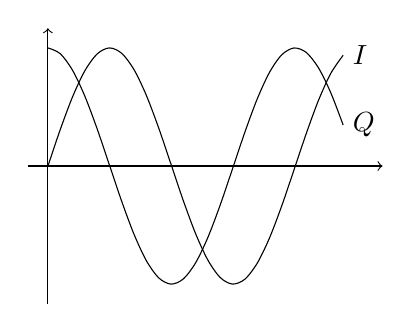
\begin{tikzpicture}[scale=0.5,domain=0:7.5,smooth]
            \draw[->] (0, -3.5) to (0, 3.5);
            \draw[->] (-0.5, 0) to (8.5, 0);
            
            \draw plot (\x, {3*cos(\x r)}) node[right] {$Q$};
            \draw plot (\x, {3*sin(\x r)}) node[right] {$I$};
        \end{tikzpicture}
    \end{center}
    
    \paragraph{Fermeture de l'Interrupteur}
    Au moment où l'on ferme l'interrupteur, l'armature gauche porte une charge $+Q_0$ et celle de droite une charge $-Q_0$. Une fois l'interrupteur fermé, le condensateur se décharge complètement, et on atteint un maximum pour $I$. Le courant continue de faire circuler les charges de l'armature gauche vers l'armature droite. Lorsque la tension devient finalement nulle, l'armature gauche du condensateur porte une charge $-Q_0$ et celle de droite une charge $+Q_0$. Le courant repart alors dans l'autre sens.
    
    \paragraph{Énergie Totale Initiale Stockée dans le Condensateur}
    \[ U_{\text{tot}} = \frac{1}{2} \frac{Q_0^2}{C} = \frac{1}{2} LI_0^2 \]
    
\end{multicols*}